% ------------------------------------------------------------------
\renewcommand{\thisunit}{MATH327 Unit 3}
\renewcommand{\moddate}{Last modified 16 Feb.~2025}
\setcounter{section}{3}
\setcounter{subsection}{0}
\phantomsection
\addcontentsline{toc}{section}{Unit 3: Canonical ensemble}
\section*{Unit 3: Canonical ensemble}
\subsection{\label{sec:reservoir}The thermal reservoir}
\subsubsection{\label{sec:replicas}Replicas and occupation numbers}
While it is reasonable to forbid particle exchange, for example by sealing gases inside airtight containers, it is not practical to prevent energy exchange as would be needed to fully isolate statistical systems.
Any thermal insulator is imperfect, and any observation of the system would require exchanging energy with the external observer. % E.g., we want to analyse a gas in a container without having to include ourselves as part of this ``system''....
In practice it is more convenient to work with physical systems that are characterized by their (intensive) temperatures rather than their (extensive) internal energies.

\begin{shaded}
  This leads us to define the \textbf{canonical ensemble} to be a statistical ensemble characterized by its fixed temperature $T$ and conserved particle number $N$, with the temperature held fixed through contact with a \textbf{thermal reservoir}.
\end{shaded}

The second part of this definition connects the fixed temperature to the fundamental fact of energy conservation (the first law of thermodynamics).
This is done by proposing that our system of interest \Om is in thermal contact with a much larger external system $\Om_{\text{res}}$ --- the thermal reservoir, sometimes called a ``heat bath''.
The overall combined system $\Om_{\text{tot}} = \Om_{\text{res}} \otimes \Om$ is governed by the micro-canonical ensemble, with conserved total energy $E_{\text{tot}} = E_{\text{res}} + E \approx E_{\text{res}}$, while the energy $E$ of \Om is allowed to fluctuate. % TODO: Could note that approximation is motivated by extensivity of energy...
The key qualitative idea is that, in thermodynamic equilibrium, \Om has a negligible effect on the overall system.
In particular, the temperature of that overall system --- and therefore the temperature of $\Om$, by intensivity --- is set by the reservoir and remains fixed even as $E$ fluctuates.
This effectively generalizes the setup we used to analyse heat exchange in the previous section, where we saw that thermal contact causes a net flow of energy from hotter systems to colder systems.
When these systems are `natural', this cools the hotter one by heating the colder one.

The mathematical implementation of this argument, as developed by Gibbs, proceeds by considering a well-motivated ansatz for the form of the thermal reservoir $\Om_{\text{res}}$.
\textcolor{green}{The goal}, which will be useful to keep in mind as we go through the lengthy analysis, is to show that the specific form of $\Om_{\text{res}}$ is ultimately irrelevant.
This will allow us to work directly with the system of interest, $\Om$, independent of the details of the thermal reservoir that fixes its temperature.

Without further ado, we take $\Om_{\text{tot}}$ to consist of many ($R \gg 1$) identical \textbf{replicas} of the system \Om that we're interested in.
All of these replicas are in thermal contact with each other, and in thermodynamic equilibrium.\footnote{The thermal contact between any two replicas can be indirect, mediated by a sequence of intermediate replicas.  This transitivity of thermodynamic equilibrium is sometimes called the \href{https://en.wikipedia.org/wiki/Zeroth_law_of_thermodynamics}{zeroth law of thermodynamics}.  It declares that if systems $\Om_A$ \& $\Om_B$ are in thermodynamic equilibrium while systems $\Om_B$ \& $\Om_C$ are in thermodynamic equilibrium, then $\Om_A$ \& $\Om_C$ must also be in thermodynamic equilibrium.}
Choosing any one of the replicas to be the system of interest, $\Om$, the other $R - 1 \approx R$ replicas collectively form the thermal reservoir $\Om_{\text{res}}$.
Assuming we want to study reasonable systems $\Om$, this ansatz ensures that $\Om_{\text{res}}$ is also reasonable, simply much larger.

An extremely small example of this setup is illustrated by the figures below, where the system of interest is just $N = 2$ spins.
For now we assume the spins are \textit{distinguishable}, so that $\downarrow\uparrow$ and $\uparrow\downarrow$ are both distinct micro-states.
This means that each individual replica has the $M = 4$ micro-states $\om_i$ defined below.
\begin{center}
  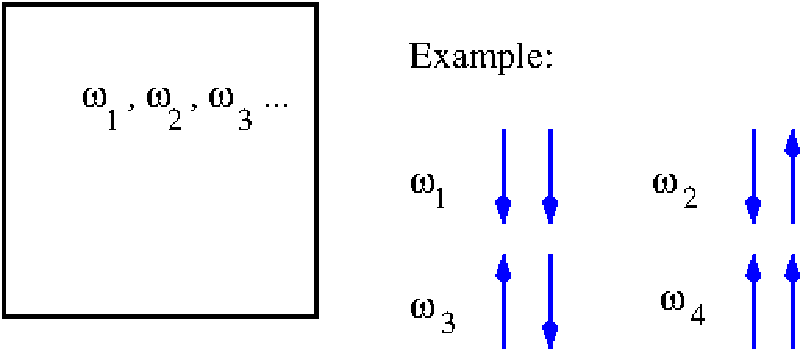
\includegraphics[width=0.7\textwidth]{figs/unit03_spin-system.pdf}
\end{center}
To form the overall system $\Om_{\text{tot}}$ we now bring together the $R = 9$ replicas shown below.
We draw boxes around each replica to remind us that they are allowed to exchange only energy with each other, while the $N = 2$ spins per replica are fixed in place.
We pick out one of these replicas (in the red box) to serve as the system \Om we will consider.
The other $8$ are the thermal reservoir $\Om_{\text{res}}$ that fixes the temperature of $\Om$.
\begin{center}
  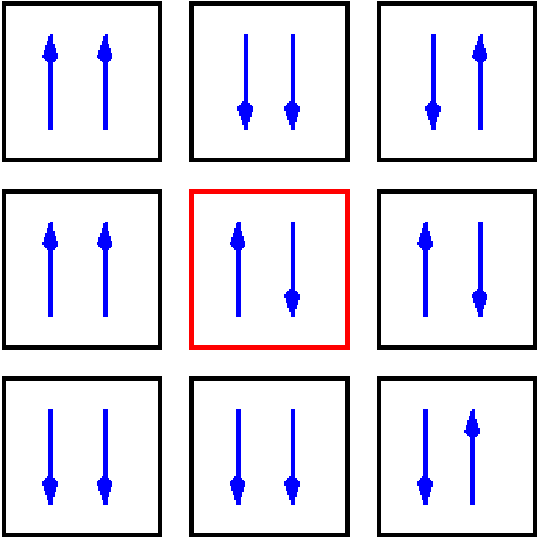
\includegraphics[width=0.7\textwidth]{figs/unit03_spin-reservoir.pdf}
\end{center}

A convenient way to analyse the overall system of $R$ replicas, $\Om_{\text{tot}}$, is to define the \textbf{occupation number} $n_i$ to be the number of replicas that adopt the micro-state $\om_i \in \Om$ in any given micro-state of $\Om_{\text{tot}}$.
The index $i \in \left\{1, 2, \cdots, M\right\}$ runs over all $M$ micro-states of $\Om$.
In the example above, three of the replicas have the micro-state $\om_1 = \downarrow\downarrow$, meaning $n_1 = 3$.
What are the occupation numbers $\left\{n_2, n_3, n_4\right\}$ for the other three $\om_i$ in the figures above?
Are all replicas are accounted for, $\sum_i n_i = R$?
\begin{mdframed}
  \ \\[50 pt]
\end{mdframed}
Normalizing the occupation number by $R$ gives us a well-defined \textit{occupation probability}, $p_i = n_i / R$ with $\sum_i p_i = 1$. % Notation anticipates that canonical probability for micro-state om_i will be p_i, since we would then expect R*p_i = n_i replicas to exhibit this micro-state...
At the moment, this $p_i$ is the probability that if we choose a replica at random it will be in micro-state $\om_i$.

Now let us consider conservation of energy, which continues to apply to the total energy $E_{\text{tot}}$ of the overall system $\Om_{\text{tot}}$.
We assume that each replica's energy $E_r$ is independent of all the other replicas.
This is guaranteed for the non-interacting systems we will focus on until Unit~9, and also holds when interactions are allowed within each replica but not between different replicas.
The thermal contact between replicas allows $E_r$ to fluctuate subject to conservation of $E_{\text{tot}}$, but there are at most $M$ possible values $E_i$ it can have, corresponding to the $M$ micro-states $\om_i \in \Om$.
Some distinct micro-states $\om_i \ne \om_j$ may have the same energy $E_i = E_j$, which doesn't affect the analysis.
This allows us to rearrange a sum over replicas into a sum over the micro-states of $\Om$:
\begin{equation}
  \label{eq:canon_Etot}
  E_{\text{tot}} = \sum_{r = 1}^R E_r = \sum_{i = 1}^M n_i E_i,
\end{equation}
with the occupation number $n_i$ counting how many times micro-state $\om_i$ appears among the $R$ replicas.
We can assume that $R$ and $M$ are both finite, so we don't need to worry about rearranging the sums.
% ------------------------------------------------------------------



% ------------------------------------------------------------------
\subsubsection{\label{sec:canon_part}Partition function}
Following Gibbs, we've taken the thermal reservoir $\Om_{\text{res}}$ to consist of $R - 1$ replicas of the system of interest, $\Om$.
The next step is to further simplify the mathematics by assuming that the overall $R$-replica system $\Om_{\text{tot}}$ is fully specified by a fixed set of $M$ occupation numbers $\left\{n_i\right\}$.
This is equivalent to assuming that the occupation probabilities $\left\{p_i\right\}$ are constant in time, as a reflection of thermodynamic equilibrium.
From \eq{eq:canon_Etot}, we see that this ensures conservation of the total energy $E_{\text{tot}}$, and we can apply the micro-canonical tools we developed in the previous unit.
Recall our ultimate \textcolor{green}{goal} of showing that such details of the thermal reservoir are irrelevant to the system $\Om$.

Based on the conservation of $E_{\text{tot}}$, we want to determine the (intensive) temperature of $\Om_{\text{tot}}$, which fixes the temperature of the system of interest, $\Om$.
According to our previous work, to do this we first need to compute the overall number of micro-states $M_{\text{tot}}$ as a function of $E_{\text{tot}}$, from which we can derive the micro-canonical entropy and temperature since the system is in thermodynamic equilibrium.
From the fixed occupation numbers $n_i$, we already know how many times each micro-state $\om_i$ appears among the $R$ replicas.
To determine $M_{\text{tot}}$ we just need to count how many possible ways there are of distributing the $\left\{n_i\right\}$ micro-states among the $R$ replicas.

If we consider first the micro-state $\om_1$, the number of possible ways of distributing $n_1$ copies of this micro-states among the $R$ replicas is just the binomial coefficient
\begin{equation*}
  \binom{R}{n_1} = \frac{R!}{n_1! \; (R - n_1)!}.
\end{equation*}
Moving on to $\om_2$, we need to keep in mind that $n_1$ replicas have already been assigned micro-state $\om_1$, so there are only $R - n_1$ replicas left to choose from.
What is the resulting number of possible ways of distributing these $n_2$ micro-states?
\begin{mdframed}
  \ \\[50 pt]
\end{mdframed}
Repeating this process for all micro-states $\left\{\om_1, \om_2, \cdots, \om_M\right\}$, recalling $\left(R - \sum_i n_i \right)! = 0! = 1$, you should obtain a product that `telescopes' to
\begin{equation}
  \label{eq:telescoped}
  M_{\text{tot}} = \frac{R!}{n_1! \; n_2! \; \cdots \; n_M!}.
\end{equation}
This confirms that the order in which we assign micro-states to replicas is irrelevant, since integer multiplication is commutative.

Thanks to thermodynamic equilibrium, the entropy of the micro-canonical $\Om_{\text{tot}}$ is
\begin{equation*}
  S(E_{\text{tot}}) = \log M_{\text{tot}} = \log(R!) - \sum_{i = 1}^M \log(n_i!),
\end{equation*}
where the dependence on $E_{\text{tot}}$ enters through the occupation numbers via \eq{eq:canon_Etot}.
With $R \gg 1$ and $n_i \gg 1$ for all $i = 1, \cdots, M$, we can approximate each of these logarithms using the first two terms in \href{https://en.wikipedia.org/wiki/Stirling's_approximation}{Stirling's formula},
\begin{align*}
  \log(N!) & = N \log N - N + \cO(\log N) \approx N \log N - N &
  \mbox{for } N & \gg 1.
\end{align*}
In order for \textit{every} occupation number to be large, $n_i \gg 1$, the number of replicas must be much larger than the number of micro-states of $\Om$.
As we have discussed before, the number of micro-states $M$ is typically a very large number, so with $R \gg M$ we are formally considering truly enormous thermal reservoirs!
This enormity helps ensure that the detailed form of the reservoir will be irrelevant.

\newpage % WARNING: FORMATTING BY HAND
Using the approximation above, what do you find for $S(E_{\text{tot}})$ in terms of $R$ and $n_i$?
What is the entropy in terms of the occupation probabilities $p_i = n_i / R$?
\begin{mdframed}
  $\displaystyle S(E_{\text{tot}}) = \log(R!) - \sum_{i = 1}^M \log(n_i!) \approx $ \\[100 pt]
\end{mdframed}
% This gives the result we would expect from extensivity.

In your result, the dependence on $E_{\text{tot}}$ now enters through the occupation probabilities $p_i$.
In order to determine the temperature, we have to express the entropy explicitly in terms of $E_{\text{tot}}$.
We do this by applying our knowledge that thermodynamic equilibrium implies maximal entropy.

Following the same steps as in \secref{sec:second_law}, we maximize the entropy, now with two Lagrange multipliers to account for two constraints on the occupation probabilities:
\begin{align*}
  \sum_{i = 1}^M p_i & = 1 &
  \sum_{i = 1}^M n_i E_i & = R \sum_{i = 1}^M p_i E_i = E_{\text{tot}}.
\end{align*}
Writing everything in terms of occupation probabilities, we therefore need to maximize the modified entropy
\begin{equation*}
  \Sbar = -R \sum_{i = 1}^M p_i \log p_i + \al\left(\sum_{i = 1}^M p_i - 1\right) - \be\left(R \sum_{i = 1}^M p_i E_i - E_{\text{tot}}\right).
\end{equation*}
Here we've chosen the sign of \be for later convenience.
What is the occupation probability $p_k$ that maximizes $\Sbar$?
\begin{mdframed}
  $\displaystyle 0 = \pderiv{\Sbar}{p_k} = $ \\[120 pt]
\end{mdframed}

\newpage % WARNING: FORMATTING BY HAND
By defining a new parameter $Z$ in terms of $\al$, you should find
\begin{equation}
  \label{eq:occ_prob}
  p_k = \frac{1}{Z} e^{-\be E_k}.
\end{equation}
As before, we need to fix the parameters $\left\{Z, \be\right\}$ by demanding that the two constraints above are satisfied.
The first of these constraints is straightforward and produces an important result:
\begin{equation}
  \label{eq:part_func}
  1 = \sum_{i = 1}^M p_i = \frac{1}{Z} \sum_{i = 1}^M e^{-\be E_i} \qquad \implies \qquad Z(\be) = \sum_{i = 1}^M e^{-\be E_i}.
\end{equation}

\begin{shaded}
  Eq.~\ref{eq:part_func} defines the canonical \textbf{partition function} $Z(\be)$, a fundamental quantity in the canonical ensemble, from which many other derived quantities can be obtained.
\end{shaded}

$Z(\be)$ still depends on the other as-yet-unknown parameter $\be(E_{\text{tot}})$.
By applying our second constraint, \eq{eq:canon_Etot}, we can relate \be to $E_{\text{tot}}$:
\begin{equation}
  \label{eq:canon_aveE}
  E_{\text{tot}} = R \sum_{i = 1}^M p_i E_i = \frac{R}{Z(\be)} \sum_{i = 1}^M E_i \; e^{-\be E_i} = R \frac{\sum_{i = 1}^M E_i \; e^{-\be E_i}}{\sum_{j = 1}^M e^{-\be E_j}}.
\end{equation}
This relation is a bit complicated, but will suffice for our goal of expressing the entropy in terms of $E_{\text{tot}}$.
Inserting \eq{eq:occ_prob} for $p_i$ into your earlier result for the entropy, what do you obtain upon applying Eqs.~\ref{eq:part_func} and \ref{eq:canon_aveE}?
\begin{mdframed}
  $\displaystyle S(E_{\text{tot}}) = -R \sum_{i = 1}^M p_i \log p_i = $ \\[100 pt]
\end{mdframed}
There is a pleasant simplification when we take the derivative to determine the temperature.
Defining $\be' \equiv \pderiv{}{E_{\text{tot}}} \be(E_{\text{tot}})$, we have
\begin{equation*}
  \frac{1}{T} = \pderiv{}{E_{\text{tot}}} S(E_{\text{tot}}) = \pderiv{}{E_{\text{tot}}} \left[E_{\text{tot}} \be + R\log Z(\be)\right] = \be + E_{\text{tot}} \be' + R \frac{1}{Z} \pderiv{Z(\be)}{\be} \be' .
\end{equation*}
Using \eq{eq:canon_aveE} we can compute
\begin{equation*}
  \frac{1}{Z} \pderiv{Z(\be)}{\be} = \frac{1}{Z} \pderiv{}{\be} \sum_{i = 1}^M e^{-\be E_i} = -\frac{1}{Z} \sum_{i = 1}^M E_i \; e^{-\be E_i} = -\sum_{i = 1}^M p_i E_i = -\frac{E_{\text{tot}}}{R},
\end{equation*}
so that we don't need to figure out the explicit form of $\be'$:
\begin{equation}
  \label{eq:beta}
  \frac{1}{T} = \be + E_{\text{tot}} \be' - E_{\text{tot}} \be' = \be .
\end{equation}

What's truly remarkable about Eqs.~\ref{eq:occ_prob}, \ref{eq:part_func} and \ref{eq:beta} is that they make no reference to the $R$ replicas or any extensive quantity of the overall system, such as $E_{\text{tot}}$ --- all information about the thermal reservoir has vanished.
This is \textcolor{green}{the goal} we have been pursuing since the start of this unit!
The large thermal reservoir is still present to fix the temperature $T$ characterizing the canonical system $\Om$, but beyond that nothing about it is relevant (or even knowable) in the canonical approach.
Every aspect of \Om can now be specified in terms of its fixed temperature $T$ and conserved particle number $N$, starting with the parameter $\be = 1 / T$.

In particular, the partition function from \eq{eq:part_func} is simply
\begin{equation}
  \label{eq:canon_part_func}
  Z(T) = \sum_{i = 1}^M e^{-E_i / T}.
\end{equation}
and together with \be specifies the probabilities
\begin{equation}
  \label{eq:canon_prob}
  p_i = \frac{1}{Z} e^{-E_i / T}
\end{equation}
from \eq{eq:occ_prob}.
This $p_i$ is now the thermodynamic equilibrium probability that \Om adopts micro-state $\om_i$ with (non-conserved) internal energy $E_i$.
This probability distribution is called either the \textbf{Boltzmann distribution} or the \textbf{Gibbs distribution}, while $e^{-E_i / T}$ itself is known as a \textbf{Boltzmann factor}.
All micro-states with the same energy have the same probability in thermodynamic equilibrium, which is consistent with the micro-canonical behaviour we saw in Unit~2.
% ------------------------------------------------------------------



% ------------------------------------------------------------------
\subsection{\label{sec:canon_derived}Internal energy, heat capacity, and entropy}
In addition to fixing the temperature of the system $\Om$, the thermal reservoir also allows the internal energy of \Om to fluctuate.
The system simply exchanges energy with the reservoir, satisfying the first law of thermodynamics.
Although the internal energy fluctuates, its expectation value $\vev{E}$ is an important derived quantity in thermodynamic equilibrium.
Applying the general definition from \eq{eq:expect_disc} to the probability space of the canonical ensemble,
\begin{equation*}
  \vev{E}\!(T) = \sum_{i = 1}^M E_i \; p_i = \frac{1}{Z} \sum_{i = 1}^M E_i \; e^{-\be E_i}.
\end{equation*}
Here we highlight the dependence of $\vev{E}$ on the temperature, and also freely interchange $\be = 1 / T$.

\newpage % WARNING: FORMATTING BY HAND
The expression above may look familiar from our work in the previous section:
\begin{mdframed}
  $\displaystyle \pderiv{}{\be} \log Z = $ \\[100 pt]
\end{mdframed}
In this case it is easier to take the derivative with respect to \be as opposed to
\begin{equation}
  \label{eq:beta_T}
  \pderiv{}{\be} = \pderiv{T}{\be} \pderiv{}{T} = -\frac{1}{\be^2} \pderiv{}{T} = -T^2 \pderiv{}{T}.
\end{equation}

In \secref{sec:temp}, we saw that `natural' micro-canonical systems exhibit higher (derived) temperatures for larger (conserved) internal energies.
Here, in the canonical approach, the average internal energy $\vev{E}$ is the derived quantity while the temperature is fixed.
From our everyday experience, we expect a similar direct relation between temperature and energy, which the following result confirms.

\begin{shaded}
  The \textbf{heat capacity} is defined to be
  \begin{equation}
    \label{eq:heat_cap}
    c_v = \pderiv{}{T} \vev{E},
  \end{equation}
  and is always non-negative, $c_v \geq 0$.
\end{shaded}

The subscript indicates that the volume of the system is kept fixed; we'll consider the role of the volume more carefully starting in Unit~4.
In a homework assignment you will confirm $c_v \geq 0$ by deriving a \textbf{fluctuation--dissipation} (or \textbf{fluctuation--response}) \textbf{relation}.
That relation will be a special case of a \href{https://en.wikipedia.org/wiki/Fluctuation-dissipation_theorem}{more general theorem}, and will connect the fluctuations of the internal energy around its expectation value, $\left(E_i - \vev{E}\right)^2$, to the energy's \textit{response} to a change in temperature, $\pderiv{}{T} \vev{E}$.
Only extremely special cases will produce $c_v = 0$, meaning that the heat capacity is generically positive, in agreement with our intuition that higher temperatures produce larger internal energies.

\newpage % WARNING: FORMATTING BY HAND
Finally, we can compute the entropy of \Om with no reference to the thermal reservoir, apart from its role fixing the temperature in thermodynamic equilibrium.
Since the general definition of the entropy in \eq{eq:entropy} continues to hold for the canonical ensemble, we just need to insert the probabilities $p_i$ from \eq{eq:canon_prob}:
\begin{mdframed}
  $\displaystyle S(T) = -\sum_{i = 1}^M p_i \log p_i = $ \\[100 pt]
\end{mdframed}
You should find that the entropy depends on $\log Z$.
% ------------------------------------------------------------------



% ------------------------------------------------------------------
\subsection{\label{sec:Helmholtz}Helmholtz free energy}
This dependence of the entropy on $\log Z$ is in accordance with our earlier claim that the partition function is a fundamental quantity in the canonical ensemble.
Recalling from \eq{eq:canon_part_func} that $Z$ is a sum over all micro-states, we can view this result as the canonical counterpart to the micro-canonical entropy being the logarithm of the number of micro-states.
(Thermodynamic equilibrium is required in both cases.)
This motivates the following definition of a quantity with the dimensions of energy that is related to $\log Z$, which provides simpler and more elegant expressions for the derived quantities we considered above.

\begin{shaded}
  The \textbf{Helmholtz free energy} of a system in the canonical ensemble is
  \begin{align}
    \label{eq:helmholtz}
    F(T) & = -T \log Z(T) &
    F(\be) & = -\frac{\log Z(\be)}{\be},
  \end{align}
  where $Z$ is the partition function of the system.
  In terms of this free energy, Eqs.~\ref{eq:canon_part_func} and \ref{eq:canon_prob} are
  \begin{align*}
    Z & = e^{-F / T} &
    p_i & = e^{(F - E_i) / T}.
  \end{align*}
\end{shaded}

\newpage % WARNING: FORMATTING BY HAND
The Helmholtz free energy is named after \href{https://en.wikipedia.org/wiki/Hermann_von_Helmholtz}{Hermann von Helmholtz} and reveals its usefulness when we take its derivative.
The derivative involves $\pderiv{}{T} \log Z$, which is worth collecting in advance based on \eq{eq:beta_T}:
\begin{mdframed}
  $\displaystyle -\pderiv{}{T}\left(\frac{F(T)}{T}\right) = \pderiv{}{T} \log Z(T) = $ \\[50 pt]
  $\displaystyle \pderiv{}{T} F(T) = $ \\[50 pt]
\end{mdframed}
From these results we can read off the more elegant expressions promised above:
\begin{align}
  S(T) & = -\pderiv{}{T} F(T) \label{eq:canon_entropy-F} \\
  \vev{E}\!(T) & = -T^2 \pderiv{}{T}\left(\frac{F(T)}{T}\right) = \pderiv{}{\be}\left[\be F(\be)\right] = T S(T) + F(T). \label{eq:canon_energy-F}
\end{align}
% ------------------------------------------------------------------



% ------------------------------------------------------------------
\subsection{\label{sec:spin_info}The physics of information}
As a first application of the canonical ensemble, we will explore physically observable effects that depend on the information content of a statistical system.
A famous scientific question illustrating the importance of information, which you may have heard of, is the \href{https://en.wikipedia.org/wiki/Black_hole_information_paradox}{black hole information paradox}.
However, that topic is well beyond the scope of this module since it depends on quantum mechanics and general relativity in addition to statistical mechanics.
Here we will consider simple spin systems as introduced in \secref{sec:ensemble}, contrasting the behaviour of their average internal energy $\vev{E}$ and entropy $S$ depending on whether or not the spins can (in principle) be distinguished from each other.
It's important to appreciate that the ``information'' discussed here is an intrinsic property of the system --- what is \textit{knowable} about it in principle.
It does not matter whether or not any observer actually knows this information; so long as it can possibly be known it will have an effect.

\subsubsection{\label{sec:spin_chain}Distinguishable spins in a solid}
We begin with the setup from \secref{sec:ensemble}: A system of $N$ spins arranged in a line, placed in an external magnetic field of strength $H$, and in thermodynamic equilibrium.
We further specify that the spins are embedded in a solid material that fixes their positions and prevents them from moving.
This allows them to be distinguished from one another: An observer can target an appropriate position in the solid to measure the corresponding spin.
Each spin measured in this way will be either parallel or anti-parallel to the magnetic field.
The canonical system therefore has $M = 2^N$ distinct micro-states $\om_i$ with energies $E_i$ and probabilities $p_i = \frac{1}{Z} e^{-E_i / T}$, each defined by the orientations of all $N$ spins.

To streamline our notation, we can represent the orientation of the $n$th spin as $s_n \in \left\{1, -1\right\}$, where $s_n = 1$ indicates alignment parallel to the field and $s_n = -1$ indicates alignment anti-parallel to the field.
With this notation, the internal energy of the system in micro-state $\om_i$ specified by the $N$ spins $\left\{s\right\}$ is simply
\begin{equation}
  \label{eq:spin_energy}
  E_i = -H \sum_{n = 1}^N s_n.
\end{equation}
To compute the canonical partition function $Z_D$, where the subscript reminds us of the spins' distinguishability, we have to sum over all $2^N$ possible spin configurations $\left\{s\right\}$.
In this process we can save some space by defining the dimensionless variable $x = \be H = \frac{H}{T}$:
\begin{align}
  Z_D & = \sum_{s_1 = \pm 1} \cdots \sum_{s_N = \pm 1} e^{-\be E_i} = \sum_{s_1 = \pm 1} \cdots \sum_{s_N = \pm 1} \exp\left[x \sum_{n = 1}^N s_n\right] \cr
      & = \sum_{s_1 = \pm 1} \cdots \sum_{s_N = \pm 1} e^{x s_1} \cdots e^{x s_N} = \left(\sum_{s_1 = \pm 1} e^{x s_1}\right) \cdots \left(\sum_{s_N = \pm 1} e^{x s_N}\right) \cr
      & = \left(\sum_{s = \pm 1} e^{x s}\right)^N = \left(e^x + e^{-x}\right)^N = \left[2\cosh\left(\be H\right)\right]^N, \label{eq:spin_part_func}
\end{align}
distributing the summations since all the spins are independent of each other.

The corresponding Helmholtz free energy
\begin{equation}
  \label{eq:dist_Helm}
  F_D(\be) = -\frac{\log Z(\be)}{\be} = -\frac{N \log\left[2\cosh\left(\be H\right)\right]}{\be}
\end{equation}
is all we need to compute the average internal energy:
\begin{mdframed}
  $\displaystyle \vev{E}_D = \pderiv{}{\be}\left[\be F_D(\be)\right] = $ \\[90 pt]
\end{mdframed}
From this we immediately obtain the entropy
\begin{equation}
  \label{eq:dist_entropy}
  S_D = \be\left(\vev{E}_D - F_D\right) = -N\be H \tanh\left(\be H\right) + N \log\left[2\cosh\left(\be H\right)\right].
\end{equation}
These results for $\vev{E}_D$ and $S_D$ are plotted on the next page as functions of $\frac{T}{H} = \frac{1}{\be H}$, using \href{https://github.com/daschaich/MATH327_2025/blob/main/lecture_notes/unit03_distinguish.py}{this Python code}.
Since both these quantities are extensive, we normalize them by showing $\frac{\vev{E}_D}{NH}$ and $\frac{S_D}{N}$.

\begin{center}
  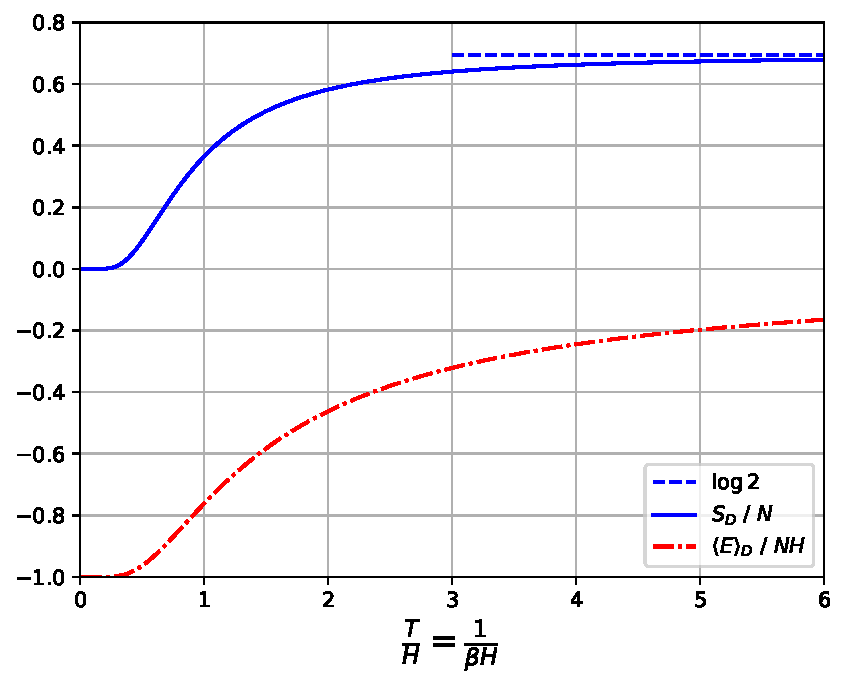
\includegraphics[width=0.9\textwidth]{figs/unit03_distinguish.pdf}
\end{center}

Let's analyse the asymptotic behaviour of these functions, starting with \textbf{low temperatures}.
In contrast to the micro-canonical \eq{eq:spin_temp}, in the canonical ensemble there is no issue with taking the independent variable $T \to 0$.
This corresponds to $\be H \to \infty$ and $\tanh\left(\be H\right) \to 1$, approaching the ``ground-state'' energy $E_{\text{min}} = E_0 = -NH$ you computed in \secref{sec:temp}.
This energy is only produced by the single micro-state in which all the spins are aligned with the magnetic field, $s_n = 1$ for all $n$ (or $n_+ = N$ and $n_- = 0$ in the notation from \secref{sec:temp}).
Correspondingly, $\log\left[2\cosh\left(\be H\right)\right] \to \log e^{\be H} = \be H$ and the two terms in \eq{eq:dist_entropy} cancel out, so that $S_D \to 0$.
This vanishing entropy is a generic consequence of temperatures approaching \textit{absolute zero}.

For low but non-zero temperatures, $\vev{E}_D$ and $S_D$ will be affected by the non-zero probability for the system to adopt micro-states $\om_i$ with higher energies $E_i > E_0$.
These higher-energy configurations are often referred to as ``excited states''.
Note that each energy $E_i > E_0$ may correspond to many different micro-states.
For example, in \secref{sec:temp} you also computed the energy $E_1 = -(N - 2)H$ of the first excited state, which is realized by the $N$ distinct micro-states with $n_- = 1$.
In the case of spin systems, we can instead refer to \textit{energy levels} that are all separated by a constant \textit{energy gap} $\De E \equiv E_{n_- + 1} - E_{n_-} = 2H$.

\newpage % WARNING: FORMATTING BY HAND
We can compute the effects of the higher energy levels at low temperatures $\be H \gg 1$ by expanding $\vev{E}_D$ in powers of $e^{-\be H} \ll 1$.
What is the first temperature-dependent term in this expansion?
\begin{mdframed}
  $\displaystyle \frac{\vev{E}_D}{NH} = $ \\[100 pt]
\end{mdframed}
You should find that the excited-state effects are \textit{exponentially} suppressed by the energy gap $\De E$ at low temperatures,
\begin{equation*}
  \frac{\vev{E}_D}{NH} = -1 + 2e^{-\be \De E} + \cO\left(e^{-2\be \De E}\right).
\end{equation*}
This is a generic feature of canonical systems with a non-zero energy gap, and is due to the exponentially suppressed probability for the system to adopt any of the micro-states with the higher energy,
\begin{equation*}
  \frac{\frac{1}{Z} e^{-\be E_{n_- + 1}}}{\frac{1}{Z} e^{-\be E_{n_-}}} = e^{-\be \De E}.
\end{equation*}

The low-temperature expansion of \eq{eq:dist_entropy} for the entropy in powers of $e^{-\be H} \ll 1$ is similar:
\begin{mdframed}
  $\displaystyle \frac{S_D}{N} = $ \\[100 pt]
\end{mdframed}
Here the leading term includes a linear factor of $\be \De E \gg 1$, but this can't overcome the now-expected exponential suppression:
\begin{equation*}
  \frac{S_D}{N} = \be \De E e^{-\be \De E} + e^{-\be \De E} + \cO\left(\be \De E e^{-2\be \De E}\right).
\end{equation*}

In the limit of \textbf{high temperatures} we should instead expand in powers of the small factor $\be H \ll 1$.
This is straightforward for $\vev{E}_D$:
\begin{equation*}
  \frac{\vev{E}_D}{NH} = -\tanh\left(\be H\right) = -\be H + \frac{\left(\be H\right)^3}{3} + \cO\left(\left[\be H\right]^5\right),
\end{equation*}
which vanishes $\sim$$\frac{1}{T}$ as $T \to \infty$.
This matches the micro-canonical behaviour we saw for this system from \eq{eq:spin_temp}, where the derived temperature diverged as the conserved energy approached zero.

For the entropy, there is a similar connection to micro-canonical behaviour at high temperatures:
\begin{mdframed}
  $\displaystyle \frac{S_D}{N} = $ \\[100 pt]
\end{mdframed}
As $\frac{T}{H} \to \infty$, the result
\begin{equation*}
  \frac{S_D}{N} = \log 2 - \frac{\left(\be H\right)^2}{2} + \cO\left(\left[\be H\right]^4\right)
\end{equation*}
approaches the asymptotic value $S_D \to N\log 2 = \log M$ for the $M = 2^N$ micro-states (with different energies).
Conceptually, in this limit the energy of each spin is negligible compared to the temperature, and the system approximately behaves as though the energy were zero for all micro-states (and hence conserved).
% ------------------------------------------------------------------



% ------------------------------------------------------------------
\subsubsection{Indistinguishable spins in a gas}
Next, let's consider nearly the same setup, with $N$ spins in thermodynamic equilibrium, in an external magnetic field of strength $H$.
The only difference is that now the spins are allowed to move, like particles in a one-dimensional gas.
We demand that they move slowly, so that we can ignore their kinetic energy and the total energy of the system continues to be given by \eq{eq:spin_energy}.
Since the spins don't interact with each other, they can freely move past each other, and even occupy the same space, making it impossible for them to be distinguished from one another. % Could remind that our starting point was noting we can't follow the motion of all the degrees of freedom...

To compute the fundamental canonical partition function (\eq{eq:canon_part_func}), we have to sum over the micro-states of the system.
These micro-states are no longer in one-to-one correspondence with the full configurations $\left\{s\right\}$ of the $N$ spins.
Because the spins are now indistinguishable, certain spin configurations also cannot be distinguished from each other.
The simplest example comes from the two-spin system considered in \secref{sec:replicas}, where the configurations $\downarrow\uparrow$ and $\uparrow\downarrow$ now both correspond to a single micro-state.
In this micro-state, we know only that one spin is $s_i = 1$ while the other is $s_k = -1$; it's not possible to distinguish which is which.

Generalizing, we can conclude that a single distinct micro-state corresponds to all possible permutations of spins with fixed $\left\{n_+, n_-\right\}$.
This means that each micro-state is now in one-to-one correspondence with the energy $E = -H(n_+ - n_-)$, which we can continue to organize as energy levels separated by a constant energy gap $\De E = 2H$.
As a quick example, enumerate the energy levels when $N = 4$ and list the spin configurations associated with the corresponding micro-states.
How many micro-states are there for $N$ spins?
\begin{mdframed}
  \ \\[120 pt]
\end{mdframed}

A convenient way to label these micro-states and energy levels is to define
\begin{equation*}
  E_k = -NH + 2Hk = -H(N - 2k)
\end{equation*}
for micro-state $\om_k$ with $k = n_- = 0, \cdots N$.
To compute the partition function $Z_I$, with the subscript reminding us about the spins' indistinguishability, we now have
\begin{equation}
  Z_I = \sum_{k = 0}^N e^{-\be E_k} = \sum_{k = 0}^N e^{\be H (N - 2k)} = e^{N\be H} \sum_{k = 0}^N \left(e^{-2\be H}\right)^k = e^{N\be H} \frac{1 - e^{-2(N + 1) \be H}}{1 - e^{-2\be H}}.
\end{equation}
The geometric series in the last step can be reconstructed by considering
\begin{equation*}
  \sum_{k = 0}^N x^k = \sum_{k = 0}^{\infty} x^k - \sum_{k = N + 1}^{\infty} x^k = \frac{1}{1 - x} - x^{N + 1} \sum_{\ell = 0}^{\infty} x^{\ell} = \frac{1}{1 - x} - \frac{x^{N + 1}}{1 - x}.
\end{equation*}

The corresponding Helmholtz free energy is
\begin{equation}
  \label{eq:indist_Helm}
  F_I(\be) = -\frac{\log Z_I(\be)}{\be} = -NH - \frac{\log\left[1 - e^{-2(N + 1) \be H}\right]}{\be} + \frac{\log\left[1 - e^{-2 \be H}\right]}{\be}.
\end{equation}
In contrast to \eq{eq:dist_Helm}, $F_I(\be)$ is no longer proportional to $N$.
In a homework assignment you will use $F_I$ to determine the average internal energy $\vev{E}_I$ and entropy $S_I$ shown in the figures on the next page, and also analyse the low- and high-temperature expansions like we did for the distinguishable case above.
Unlike our results for the distinguishable case, you will find that $\frac{\vev{E}_I}{NH}$ and $\frac{S_I}{N}$ depend on $N$, which requires us to fix $N = 4$ in the plots on the next page.
\begin{center} % Don't need centering, but this will provide consistent vertical spacing
  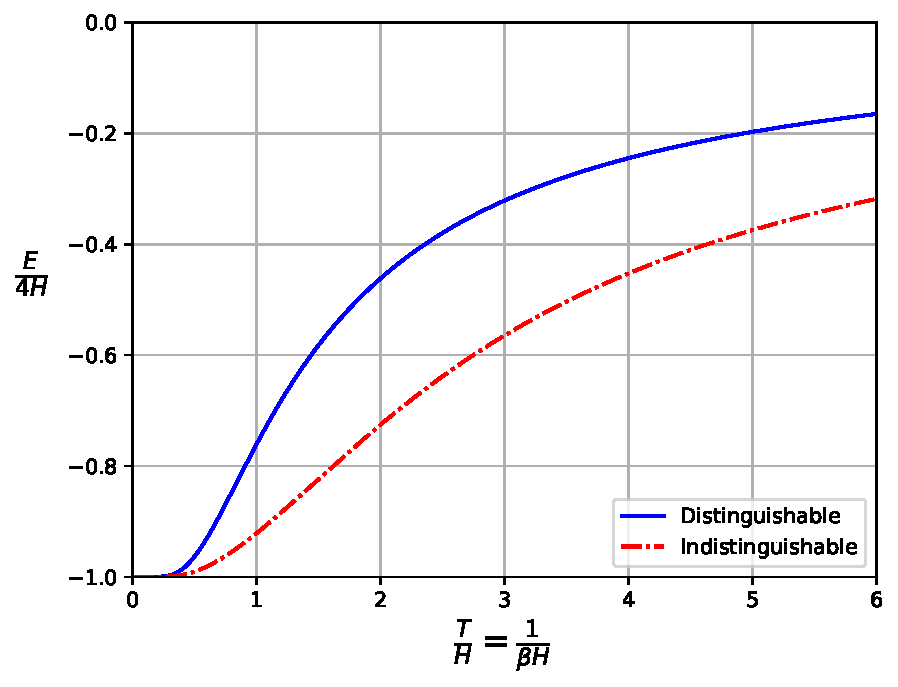
\includegraphics[width=0.475\textwidth]{figs/unit03_energies.pdf}\hfill 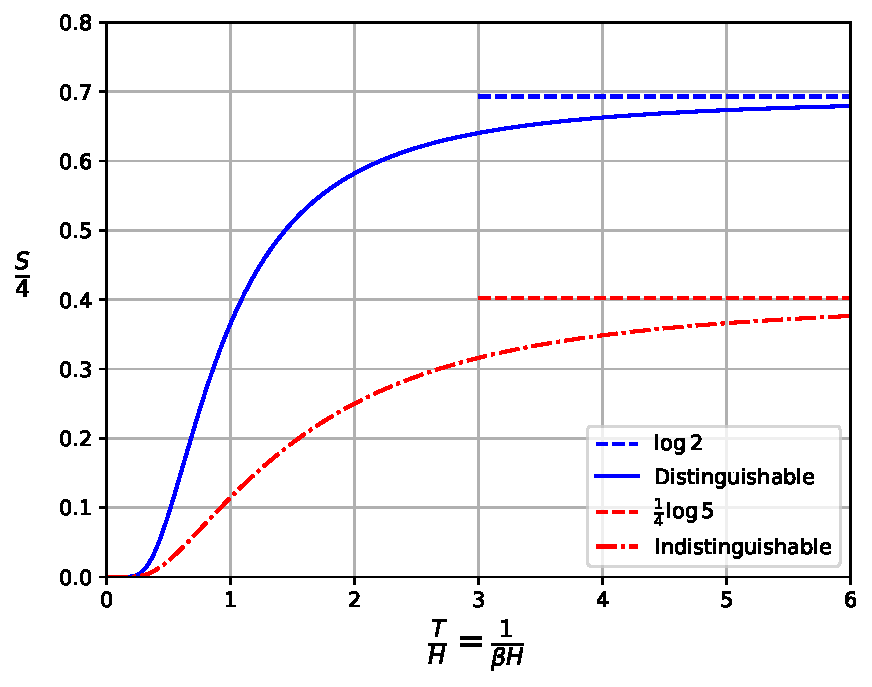
\includegraphics[width=0.475\textwidth]{figs/unit03_entropies.pdf}
\end{center}

The solid blue lines in these figures are exactly the distinguishable-spin results we previously discussed.
The red dash-dotted lines are the new results for indistinguishable spins.
We see that the same $T \to 0$ limits are approached in both cases: $E \to -NH$ and $S \to 0$.
At low temperatures, the indistinguishable results approach these limits more quickly --- they still feature exponential suppression of excited-state effects by the energy gap, $\propto$$e^{-\be \De E}$, but this now comes with additional factors of $N$.

At high temperatures there is an even more striking difference.
While the average internal energy $\vev{E}_I$ continues to vanish $\sim$$\frac{1}{T}$ as $T \to \infty$ (with different $N$ dependence), the entropy approaches the asymptotic value $S_I \to \log\left(N + 1\right) = \log M$ for the $M = N + 1$ micro-states.
This logarithmic dependence on $N$ is very different from the $S_D \to N\log 2$ limit we found for distinguishable spins, and reflects the exponentially smaller number of micro-states that exist for indistinguishable spins, $N + 1$ vs.\ $2^N$.

Finally, away from those low- and high-temperature limits, the left figure above shows a significant difference in the internal energies of the spin systems, depending only on whether or not the spins can be distinguished from each other in principle.
This is a physically measurable effect caused by the intrinsic information content of a statistical system, and a simple illustration of phenomena that remain at the leading edge of ongoing research.
As \href{https://en.wikipedia.org/wiki/Rolf_Landauer}{Rolf Landauer} put it in a famous 1991 essay: \href{https://scottaaronson.blog/?p=3327}{Information is physical}.
% ------------------------------------------------------------------
